\documentclass[12pt]{article}
\usepackage{amsmath}
\usepackage{amssymb}
\usepackage{fancyhdr}
\usepackage{graphicx}
\usepackage{pdfpages}
\usepackage{listings}
\usepackage{color}
\usepackage{lmodern}
\usepackage{hyperref}

\definecolor{dkgreen}{rgb}{0,0.6,0}
\definecolor{gray}{rgb}{0.5,0.5,0.5}
\definecolor{mauve}{rgb}{0.58,0,0.82}
\pagestyle{headings}
\setlength{\oddsidemargin}{0in}
\setlength{\evensidemargin}{0in}
\setlength{\textheight}{9in}
\setlength{\textwidth}{6.5in}
\setlength{\topmargin}{-0.5in}
\setlength{\headheight}{14pt}
\renewcommand*\rmdefault{lmss}
\renewcommand*\contentsname{Table of Contents}
\lstset{language=Matlab,
	aboveskip=3mm,
	belowskip=3mm,
	showstringspaces=false,
	basicstyle={\normalfont\ttfamily},
	numbers=left,
	numberstyle=\tiny\color{gray},
	keywordstyle=\color{blue},
	commentstyle=\color{dkgreen},
	stringstyle=\color{mauve},
	breaklines=true,
	breakatwhitespace=true,
	tabsize=4
}

\newcommand{\horizontalLine}{
	\begin{center}
		\hrule width 1.0\textwidth
	\end{center}
}

\newcommand{\smallHorizontalLine}{
    \begin{center}
        \hrule width 0.5\textwidth
    \end{center}}

%%%%%%%%%%%%%%%%%%%%%%%%%%%%%%%%%%%%%%%%%%%%%%%%%%%%%%%%%%
%%%%%%%%%%%%%%%%%%%%%%%%%%%%%%%%%%%%%%%%%%%%%%%%%%%%%%%%%%
\title{\vspace{-3ex}\bf Final Project Report\\[2ex] 
       \normalsize ECS 171: Machine Learning\\Fall 2015}
\date{\today}
\author{\bf Team Name: The Muses\\ \bf William Otwell (997371020)\\ \bf Marshall Hampson (998795016)\\ \bf Nicholas Layton (996933702)\\ \bf Steven Mackey ()\\ \bf James Dryden (993083613)\\ \bf Amos Too (998124687)\\ \bf Michael Fiueroa (998378271)\\ \bf Peggy Li (998440170)}
%%%%%%%%%%%%%%%%%%%%%%%%%%%%%%%%%%%%%%%%%%%%%%%%%%%%%%%%%%
%%%%%%%%%%%%%%%%%%%%%%%%%%%%%%%%%%%%%%%%%%%%%%%%%%%%%%%%%%
\begin{document}
\maketitle
\pagebreak
\tableofcontents
\pagebreak
%%%%%%%%%%%%%%%%%%%%%%%%%%%%%%%%%%%%%%%%%%%%%%%%%%%%%%%%%%
%%%%%%%%%%%%%%%%%%%%%%%%%%%%%%%%%%%%%%%%%%%%%%%%%%%%%%%%%%
\section{Abstract}
\label{sec:abstract}
Music lovers worldwide are in constant search of new sounds to enrich their music library. Many analytic applications have risen to popularity as a result of listeners' need for music discovery. Most of these applications utilize machine learning techniques to make recommendations and predictions for their users. One of the more common problems in music analytics is the process of recommending an enjoyable song or artist to a user based on their previous music choices. Another popular problem is the process of generating a personalized playlist for a user, again based on their listening choices. We sought to solve similar problems by performing predictive analytics on songs based on their acoustic qualities. We hoped to discover any relationship between a song's acoustic qualities and its inaudible qualities, such as genre or popularity. 
%%%%%%%%%%%%%%%%%%%%%%%%%%%%%%%%%%%%%%%%%%%%%%%%%%%%%%%%%%
%%%%%%%%%%%%%%%%%%%%%%%%%%%%%%%%%%%%%%%%%%%%%%%%%%%%%%%%%%
\horizontalLine
\section{Introduction}
\label{sec:introduction}
%%%%%%%%%%%%%%%%%%%%%%%%%%%%%%%%%%%%%%%%%%%%%%%%%%%%%%%%%%
\subsection{Background}
\label{subsec:background}
The motivation to develop "smarter" software for music analytics originates largely from a desire to sell more products to customers. Some of the biggest players in the industry, Amazon and Apple, are notoriously known for their "genius" recommendations on what customers ought to buy next. Brian Whitman, co-founder and CTO of the Echo Nest, said in his article titled \textit{How music recommendation works - and doesn't work} that, "Amazon is not optimizing for the noble work of raising independent artists' profiles to the public, and they're definitely not optimizing for a good musical experience. They're statistically optimizing to make more money, to sell you more things." Although many companies have found success using this technique, Brian expresses the importance of not only focusing on these money-making optimizations but also satisfying listeners by focusing on the actual music, its sound waves and lyrical significance. He believes that the sound of a song can contribute much more to predictive analytics than users' purchase history or song popularity.

Our approach to music analytics was similar to that of Brian Whitman's company, minus the lyrical analysis. We utilized data that represented the actual sound of the music, an approach that Brian calls "acoustic analysis." Some of the features that we included in our analysis, for example, were time signature, loudness, and key, to name a few. We hoped to focus our analysis on the sounds of the music and how the features of a song itself could provide predictive information. More specifically, the goals we hoped to accomplish were:
\vspace{-3.5mm}
\begin{itemize}
    \item Predict the popularity of a song by applying linear regression techniques to quantify and predict the popularity of a song based on its acoustic features
    \vspace{-3.5mm}
    \item Classify a song into its genre(s) by utilizing artificial neural networks to learn about the potential relationship between a song's acoustic qualities and its associated genres 
    \vspace{-3.5mm}
    \item Discover trends in the songs regarding hotness and genre by utilizing clustering techniques to discover trends in a songs features that might indicate a songs "hotness"
    \vspace{-3.5mm}
\end{itemize}
%%%%%%%%%%%%%%%%%%%%%%%%%%%%%%%%%%%%%%%%%%%%%%%%%%%%%%%%%%
\subsection{Million Song Dataset}
\label{subsec:datasetIntro}
The dataset that we chose to use is known as the Million Song Dataset (see Appendix~\ref{subsec:datasetsAndCode} for more info). Rather than actually using 1 million songs, we used a small, manageable subset of the Million Song Dataset. The features that we used were: danceability, duration, end-of-fade-in, energy, key, loudness, mode, song-hotness, start-of-fade-out, tempo, time-signature, year, and artist-terms, which is simply a list of tags (which in our case can be thought of as genres) for each song.
%%%%%%%%%%%%%%%%%%%%%%%%%%%%%%%%%%%%%%%%%%%%%%%%%%%%%%%%%%
%%%%%%%%%%%%%%%%%%%%%%%%%%%%%%%%%%%%%%%%%%%%%%%%%%%%%%%%%%
\horizontalLine
\section{Methods}
\label{sec:methods}
%%%%%%%%%%%%%%%%%%%%%%%%%%%%%%%%%%%%%%%%%%%%%%%%%%%%%%%%%%
\subsection{Linear Regression}
\label{subsec:linearRegression}
In an effort to study the predictability of song "hotness" (a measure of popularity included in our data), we used linear regression and various feature sets to create a working model. We began with feature reduction, using Lasso regression and Principal Component Analyses followed by normal linear regression. We began modeling with the above listed features, but with danceability and energy ignored. We also selectively used elements with a listed hotness of zero. Such an absolute value suggests missing data more than complete dearth of popularity, so we removed it in some models. This greatly reduced the resulting error. We also tested the use of different numbers of song tags, testing with the more popular genres. We represented these song tags as a matrix of binary indicators, in which the rows are associated with sample and the columns with the different song tags.

%%%%%%%%%%%%%%%%%%%%%%%%%%%%%%%%%%%%%%%%%%%%%%%%%%%%%%%%%%%%%
\subsection{Artificial Neural Networks}
\label{subsec:ann}
We utilized Neural Networks to predict song genres based on features of a song. Many songs, however, belonged to several genres. To represent the various genres, also known as tags, for a particular song, we formed an $m \times k$ matrix of 0s to represent the tags for all songs, where $m$ was the number of samples and $k$ was the number of possible tags. Then, we iterated through all $m$ samples to check the tags of each song, and set the indices to 1s in the tag matrix for the tags to which the current sample/song belonged.By having 12 song features and $k$ possible genres, we knew we would need to construct a neural network with 12 input nodes and $k$ output nodes. 

After determining the input and output configurations of the neural network, we became mostly with testing the effect of 3 different parameters on the neural network: learning rate, number of hidden layers, and number of hidden nodes per hidden layer. We planned to run our dataset through various neural networks, each with a different configuration of the above parameters. By doing so, we hoped to find both an optimal network configuration and a correlation between a song's features and its tags. 
%%%%%%%%%%%%%%%%%%%%%%%%%%%%%%%%%%%%%%%%%%%%%%%%%%%%%%%
\subsection{Clustering}
\label{subsec:clustering}
We took two different approaches to clustering our data: k-means and hierarchical. We looked at k-means to try and see if there had any obvious patterns and then see if those patterns held any significance for genre or song hotness. The hierarchical approach is intended to give us insight to the distribution of our data and help us select the appropriate number of clusters for k-means. For both approaches we chose to use MATLAB and take advantage of the built-in clustering methods.

For K means and hierachical, we used the subset of data mentioned previously. We noticed that danceability and energy where all 0 in the provided dataset although the value was supposed to range between 0 and 1. Therefore we decided to not use these features in our clustering. We also removed year and mode because the ended up being nearly categorical: their normalized values were almost 0 or almost 1. Finally, We also only used the samples that had a value for hotness as many were set to 0 indicating no data. 

For k-means clustering we ran our reduced data through the MATLAB k-means function and plotted of all these features plotted against song hotness. We started with a guidline to use sqrt(n/2) clusters. We ran k-means using this guidline, producing 44 clusters. We tried using various other numbers of clusters and decided to display results using only 4 clusters.

%%%%%%%%%%%%%%%%%%%%%%%%%%%%%%%%%%%%%%%%%%%%%%%%%%%%%%%%%
%%%%%%%%%%%%%%%%%%%%%%%%%%%%%%%%%%%%%%%%%%%%%%%%%%%%%%%%%%
\horizontalLine
\section{Results}
\label{sec:results}
%%%%%%%%%%%%%%%%%%%%%%%%%%%%%%%%%%%%%%%%%%%%%%%%%%%%%%%%%%
\subsection{Linear Regression}
\label{subsec:linearRegressionResults}
The feature sets we elected to work with were a combination of the original data set, subsets of the song tags data field, and some attempts at cleaning up the elements used in training. The first thing we tried was feature selection using Lasso regression and all features and all song tags. The resulting MSE was the highest of all trials: 0.25. The next feature reduction strategy we used was Principal Component Analyses with a second highest error of 0.0488. Looking at the scatter plot of predicted vs actual values, we see two clear aggregated bands of points. These two bands show up in normal linear regression using all features as well, but not so neatly packed together.

Our following trials involved testing the number of song tags to include as features. We found a sorted list of the most prevalent tags in the data and modeled using 20 or 5 of them. The results here were very close, though using 20 did come out slightly more accurate in ten fold cross validation. All our tests that did not include song tags had a MSE close to 0.04, while those that did include song tags hovered closer to 0.02. The final thing we tried was to eliminate row elements with a hotness rating of 0.0. This showed measurable improvement. In the final model we used the original feature set (excluding danceability and energy as these values were all zero), the top 20 song tags, and no zero valued elements. The resulting MSE was 0.0223.

We can see the relative errors of the different models in the bar graph. On the left we see the MSE with Lasso regression. The next three are the errors associated with normal linear regression with song tags included. The lower two are corrected for zero values. The three on the right are associated with no song tags (see Appendix~\ref{subsec:MSE}).
%%%%%%%%%%%%%%%%%%%%%%%%%%%%%%%%%%%%%%%%%%%%%%%%%%%%%%%%%%%%%
\subsection{Artificial Neural Networks}
\label{subsec:annResults}
We found that the number of output nodes negatively impacted our experimental results. Including all of the possible tags from our dataset yielded extremely undesirable results. Furthermore, computational overhead of training with all 300 outputs resulted in very long wait times between training runs. Instead, we found that limiting the number of possible genres improved both the training error and misclassification rate. Initially, we constructed our network with 12 input nodes and $k = 301$ output nodes. We then attempted to iterate through various configurations of hidden layers, hidden nodes, and learning rates, but found that none of them yielded results anywhere remotely near desirable. Both the training error and misclassification rate would consistently skyrocket, regardless of the learning rate or hidden layer/node configuration.

After considering our options for improving the performance of our network, we resorted to limiting the maximum number of output nodes to $k = 5$. We only considered genres that belonged to the top 5 genres from our list of most popular genres, which were: rock, electronic, pop, alternative rock, and hip hop. Songs that didn't belong to any of these genres were not classified into any category. Although, this approach dramatically improved the performance of our network, it still did not yield a desirable training error.

Ultimately, we found that the lowest possible number of output nodes would yield the most optimal results. We chose to limit the output nodes to only the most popular genre: rock. We tested various network configurations to discover the optimal hidden-layer and learning rate configuration. The results of this experiment are illustrated in Appendix~\ref{subsec:variousANN}, which is a plot of both training error and misclassification rate for each network configuration. From this plot, we see that the optimal configuration is the 7th network: 4 hidden layers, each with 12 hidden nodes, with a learning rate of 0.05. We consider this to be the optimal network because it yields the lowest training error, which was 0.68598.
%%%%%%%%%%%%%%%%%%%%%%%%%%%%%%%%%%%%%%%%%%%%%%%%%%
\subsection{Clustering}
\label{subsec:clusteringResults}
We found that the clusters seemed to be skewed by issues with our data set. Plotting our data before removing year and mode skewed our data into clusters based only on these two features. Before removing the bad from hotness, our clusters were all significantly shifted towards zero hotness. However, our data did not split into zero hotness clusters vs non zero hotness clusters. All the clusters were shifted down equally. After removing these features and a set of incomplete elements from the dataset, we found we got more distinct clusters. Below is our k-means clustering with four clusters, both before and after removing features.
See Appendix~\ref{subsec:trimmedKmeans} and Appendix~\ref{subsec:untrimmedKmeans}


We compared our hierarchical dendrogram to that of a randomly generated sample. They showed a very similar structure. Comparing the distance values from the dendrograms, we found that there were really 4 distinct leaves in our data. After the 4 initial splits, future splits didn't look any more significant than they would in a dendrogram for random data. Below are the dendragrams from our data and one of random data.
Refer to Appendix~\ref{subsec:dendrograms} for the dendrograms from our data and one of random data.
%%%%%%%%%%%%%%%%%%%%%%%%%%%%%%%%%%%%%%%%%%%%%%%%%%%%%%%%%%
%%%%%%%%%%%%%%%%%%%%%%%%%%%%%%%%%%%%%%%%%%%%%%%%%%%%%%%%%%  
\section{Discussion}
\label{sec:discussion}
%%%%%%%%%%%%%%%%%%%%%%%%%%%%%%%%%%%%%%%%%%%%%%%%%%
\subsection{Linear Regression}
\label{subsec:linearRegressionDisc}
The likely reason for the higher error with feature reduction is overfitting. We can see this in a scatter plot of actual vs predicted results. Regression with PCA attempts to fit the data into a very specific two band shape. It is further apparent that genre is a very important part of our regression model. This could be based on the dataset itself and the accuracy of genre attribution to a song or artist, or it could simply be that certain genres dominate the industry at different times. But even this result leads to surprisingly accurate predictions, with a MSE of 0.0223, when hotness only ranges between zero and one.

We also found correlation between features; for example certain genres are associated with different keys. These are correlations that may be obvious to a musician or professional, but not to casual consumers.We could quickly shift our methods to study these relationships as well.
%%%%%%%%%%%%%%%%%%%%%%%%%%%%%%%%%%%%%%%%%%%%%%%%%%
\subsection{Artificial Neural Networks}
\label{subsec:annDisc}
The primary obstacle in successfully constructing a predictor for song genres was the number of genres that our network was trying to simultaneously predict. As stated in Section~\ref{subsec:annResults}, we had to reduce the number of genres from 300 to 5, and then from 5 to 1 to obtain acceptable results. In many of the cases when we found ways to improve our results, we were able to reduce the training error but weren't able to reduce the misclassification rate. We think this because of the manner in which the DeepLearningToolbox (see Appendix~\ref{subsec:datasetsAndCode} for more info about the toolbox) interprets a misclassification. 

Consider the case where we are trying to predict all 300 of the top genres. Our dataset would be organized as discussed in Section~\ref{subsec:ann}, where $n = 12$ and $k = 300$. This results in an ANN of 12 inputs, and 300 outputs. If the neural network correctly classifies 299 of the 300 genres, then the overall network performed a misclassification, even though it only missed a correct classification by 1 output out of 300. This makes it very easy for the network to misclassify a sample. By reducing the number of outputs to 5 and to 1, the network has a much lower possibility of misclassifying any of the particular outputs. 

The inability to train a network with 300 output nodes could either be that a one-to-many correlation does not exist between a song's feature and the set of genres, or the complexity of a neural network with 300 output nodes is just too great to handle. One of the untested options that we think could help with classifying 300 outputs would be to construct a neural network for each output, rather than having a single network for all outputs. 
%%%%%%%%%%%%%%%%%%%%%%%%%%%%%%%%%%%%%%%%%%%%%%%%%%
\subsection{Clustering}
\label{subsec:clusteringDisc}
By examining how our data clustered we hoped to find some hint as to what features were the most significant in predicting the genre or hotness of a song.
However, after examining the visualizations of the clusters there was not much to be gained by clustering. There were no obvious relationships between
the features and genre or song hotness when we used k-means to cluster the data. Hierarchical clustering seemed to reveal slightly more; at least, it was slightly more significant than hierarchical clustering on random data. This led us to conclude that using these features were not a good choice for 
determining a songs genre. 

After we realized that this didn't yield any useful information about a songs genre, we wondered what would. In the paper, "Pandoras Music
Recommender", it seems even Pandora was not able to classify music entirely by looking at features that could be calculated from audio data like in 
our approach. Rather Pandora employees a team of musicians to "[listen to a] collection of songs and tagging each according to
approximately 400 musical attributes" (Howe 2). However, they do employ clustering algorithms in order to create groups of users with certain preferences and
to cluster songs based on similarity of the human-provided tags.
So essentially, Pandora still relies on humans analyzing what genre and musical attributes have in common, but takes advantage of machine learning techniques
to predict the next song to play, by calculating the musical "distance" between songs as well as grouping users together to generate better song predictions.
%%%%%%%%%%%%%%%%%%%%%%%%%%%%%%%%%%%%%%%%%%%%%%%%%%%%%%%%%%
%%%%%%%%%%%%%%%%%%%%%%%%%%%%%%%%%%%%%%%%%%%%%%%%%%%%%%%%%%
\horizontalLine
\section{Conclusion}
\label{sec:conclusion}
We set out to discuss modeling strategies and prediction techniques in commercial music. To create a reliable and accurate model would create opportunities not only for retailers and web radio, but for artists and consumers as well. Artists could better tailor their music to their audience, and consumers would have an accurate and helpful way of finding music similar to their interests. What we found, however, is that this task is not only characterized by a large and complicated feature set, but also very prone to randomness and noise. As the models become more complicated, the computation becomes limiting and the results often do not improve (or in some cases worsen).

Furthering this study would require the addition of big data capability and an ever changing model of current trends in music. Using a combination of proper feature selection based on current popularity and a database of purchase information, we could construct a more complicated and accurate model. Among the trends that we discovered were the importance of popular genres (as our ANN group found with the rock genre) and the danger of overfitting based on poor feature selection (as or linear regression group found with PCA). In future related work we will know how to properly avoid these pitfalls.
%%%%%%%%%%%%%%%%%%%%%%%%%%%%%%%%%%%%%%%%%%%%%%%%%%%%%%%%%%
%%%%%%%%%%%%%%%%%%%%%%%%%%%%%%%%%%%%%%%%%%%%%%%%%%%%%%%%%%
\horizontalLine
\section{References}
\label{sec:references}
%%%%%%%%%%%%%%%%%%%%%%%%%%%%%%%%%%%%%%%%%%%%%%%%%%%%%%%%%%
\subsection{Readings}
\label{subsec:readings}
\begin{enumerate}
    \item Howe, Michael. "Pandora's Music Recommender." Computer Science and Engineering. University of Washington. Web.\\ $<$\href{http://courses.cs.washington.edu/courses/csep521/07wi/prj/michael.pdf}{http://courses.cs.washington.edu/courses/csep521/07wi/prj/michael.pdf}$>$.\vspace{-1ex}
    
    \item Whitman, Brian. "How Music Recommendation Works - and Doesn't Work." Brian Whitman. Web. $<$\href{http://notes.variogr.am/post/37675885491/how-music-recommendation-works-and-doesnt-work}{http://notes.variogr.am/post/37675885491/how-music-recommendation-works-and-doesnt-work}$>$.\vspace{-1ex}

    \item Glaser, W.T, T.B. Westergren, J.P. Stearns, and J.M. Kraft. "Consumer Item Matching Method and System." Google Books. Google Patents, 21 Feb. 2006. Web.\\ $<$\href{http://www.google.com/patents/US7003515?dq=7,003,515}{http://www.google.com/patents/US7003515?dq=7,003,515}$>$.\vspace{-1ex}
    
    \item Visalakshi, N. Karthikeyani, and K. Thangavel. "Impact of Normalization in Distributed K-Means Clustering." International Journal of Soft Computing. Medwell Journals, 2009. Web. $<$\href{http://www.medwelljournals.com/fulltext/?doi=ijscomp.2009.168.172}{http://www.medwelljournals.com/fulltext/?doi=ijscomp.2009.168.172}$>$.\vspace{-1ex}
    
    \item Bergstra, James, Michael Mandel, and Douglas Eck. "SCALABLE GENRE AND TAG PREDICTION WITH SPECTRAL COVARIANCE." ISMIR 2010 Utrecht: International Society for Music Information Retrieval Conference. International Society for Music Information Retrieval Conference. Web. $<$\href{http://ismir2010.ismir.net/proceedings/ismir2010-86.pdf}{http://ismir2010.ismir.net/proceedings/ismir2010-86.pdf}$>$.\vspace{-1ex}
    
    \item Miotto, Riccardo, Luke Barrington, and Gert Lanckriet. "IMPROVING AUTO-TAGGING BY MODELING SEMANTIC CO-OCCURRENCES." ISMIR 2010 Utrecht: International Society for Music Information Retrieval Conference. International Society for Music Information Retrieval Conference. Web. $<$\href{http://ismir2010.ismir.net/proceedings/ismir2010-51.pdf}{http://ismir2010.ismir.net/proceedings/ismir2010-51.pdf}$>$.\vspace{-1ex}
    
    \item Serra, Joan, Alvaro Corral, Marian Boguna, and Martin Haro. "Measuring the Evolution of Contemporary Western Popular Music." Nature.com: Scientific Reports. Nature Publishing Group. Web. $<$\href{http://www.nature.com/articles/srep00521}{http://www.nature.com/articles/srep00521}$>$.\vspace{-1ex}
    
    \item Ni, Yizhao, Raul Santos-Rodriguez, Matt Mcvicar, and Tijl De Bie. "Hit Song Science Once Again a Science?" Research Homepage - Tijl De Bie. Tijl De Bie. Web. $<$\href{http://www.tijldebie.net/system/files/MML2011-final.pdf}{http://www.tijldebie.net/system/files/MML2011-final.pdf}$>$.
    \vspace{-1ex}
     
    \item Downie, J. Stephen. ``The music information retrieval evaluation exchange (2005-2007): A window into music information retrieval research." Acoustical Science and Technology 29.4 (2008): 247-255. $<$ \href{https://www.jstage.jst.go.jp/article/ast/29/4/29\_4\_247/\_article}{https://www.jstage.jst.go.jp/article/ast/29/4/29\_4\_247/\_article} $>$. 
    \vspace{-1ex}
    
    \item Kar, Amlan, Chaitanya Ahuja, and Amitabha Mukherjee. "Music Classification using DNN'." (2015). $<$\href{http://home.iitk.ac.in/~chahuja/cs365/project/report.pdf}{http://home.iitk.ac.in/~chahuja/cs365/project/report.pdf}$>$.

   
\end{enumerate}
%%%%%%%%%%%%%%%%%%%%%%%%%%%%%%%%%%%%%%%%%%%%%%%%%%%%%%%%%%
\subsection{Datasets and Code}
\label{subsec:datasetsAndCode}
\begin{itemize}
    \item \textbf{Million Song Dataset}: 
    \subitem Thierry Bertin-Mahieux, Daniel P.W. Ellis, Brian Whitman, and Paul Lamere. 
    The Million Song Dataset. In Proceedings of the 12th International Society
    for Music Information Retrieval Conference (ISMIR 2011), 2011. Official website by Thierry Bertin-Mahieux,
    available at: \href{http://labrosa.ee.columbia.edu/millionsong/}{http://labrosa.ee.columbia.edu/millionsong/}\vspace{-1ex}
    
    \item \href{https://github.com/rasmusbergpalm/DeepLearnToolbox}{\textbf{DeepLearningToolbox}} - Rasmus Berg Palm
    \subitem Used for the construction, configuration, training, and testing of our Artificial Neural Networks. The training algorithm uses a form of Batch Gradient Descent by constructing "mini-batches" at each iteration of training. Code available at:\\ \href{https://github.com/rasmusbergpalm/DeepLearnToolbox}{https://github.com/rasmusbergpalm/DeepLearnToolbox}\vspace{-1ex}
\end{itemize}

%%%%%%%%%%%%%%%%%%%%%%%%%%%%%%%%%%%%%%%%%%%%%%%%%%%%%%%%%%
%%%%%%%%%%%%%%%%%%%%%%%%%%%%%%%%%%%%%%%%%%%%%%%%%%%%%%%%%%
\appendix
\section{Figures}
\label{sec:figures}
\subsection{Performance of Linear Regression Models}
\label{subsec:MSE}
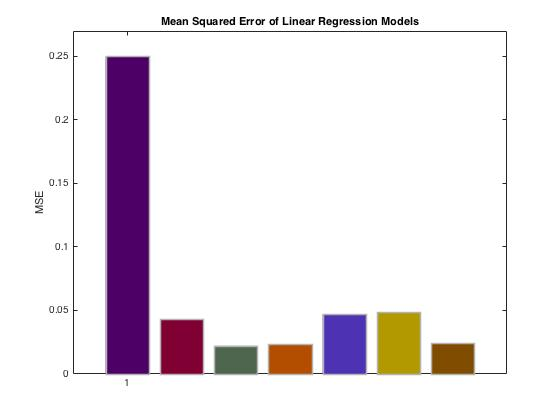
\includegraphics[scale=.5]{images/lr/mse}
\subsection{Comparison of Various Neural Network Configurations}
\label{subsec:variousANN}
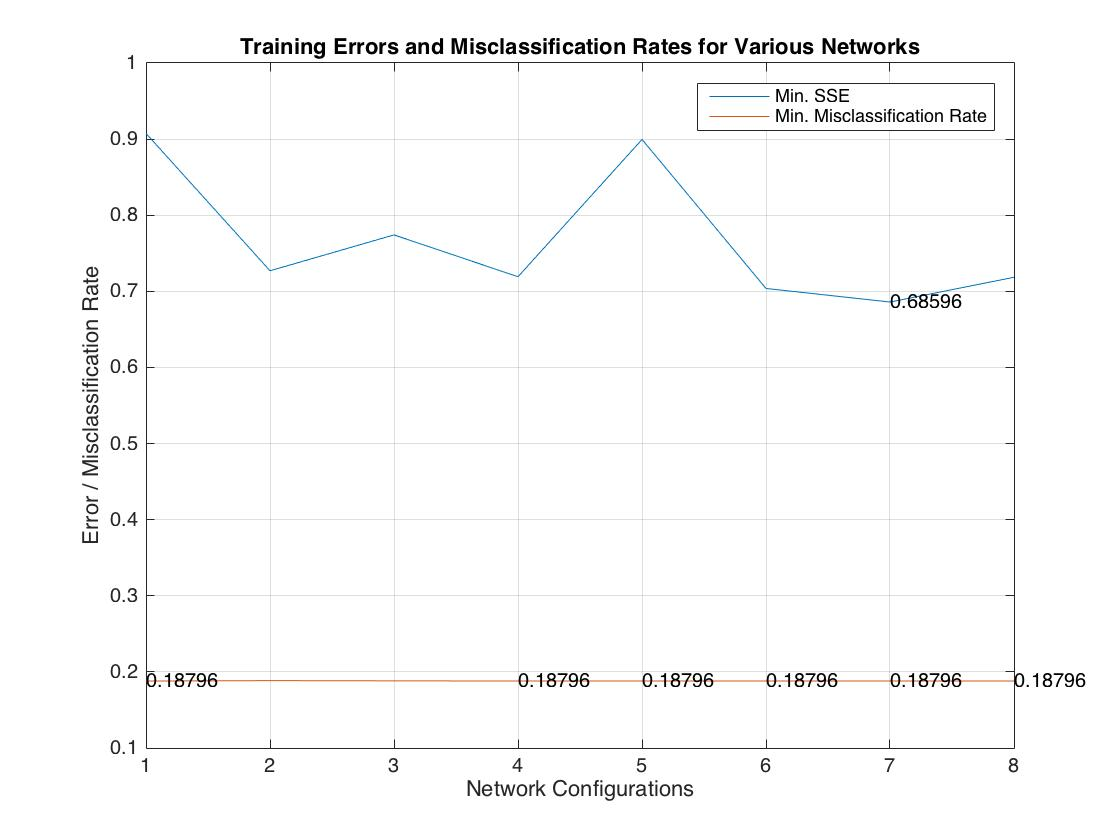
\includegraphics[scale=0.3]{images/ann/graphOfVariousNetworksWith1Genre}
\\
Each of the networks that were tested to yield the graph above contained 12 input nodes and a single output node for the classification of rock songs. The first four networks above contained 3 hidden layers, while the others contained 4. Also, the first, second, fifth, and sixth networks contained 9 hidden nodes, while the others contained 12. Finally, all of the even-numbered networks used a learning rate of 0.05, while the others used a rate of 0.1.
\subsection{K-means with features removed}
\label{subsec:trimmedKmeans}
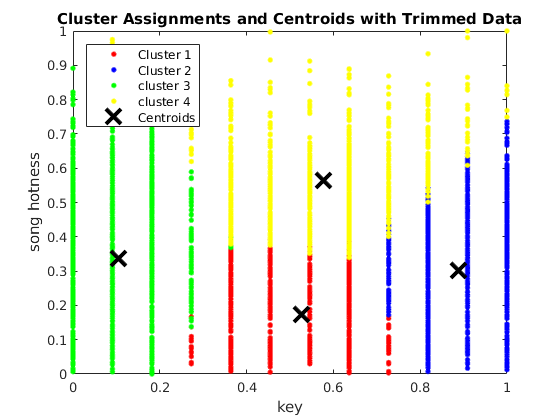
\includegraphics[scale=0.6]{images/clustering/trimmedkMeans}
\subsection{K-means without removing features}
\label{subsec:untrimmedKmeans}
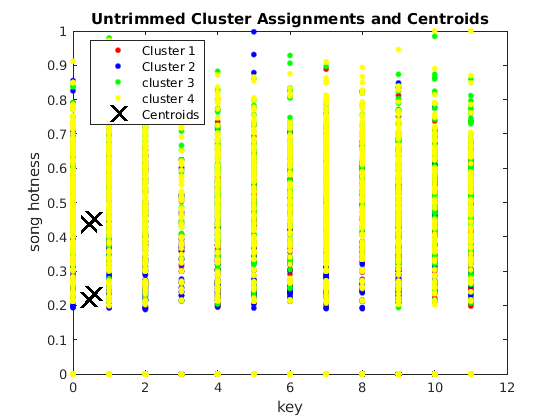
\includegraphics[scale=0.6]{images/clustering/untrimmedkmeans}
\subsection{Dendrograms}
\label{subsec:dendrograms}
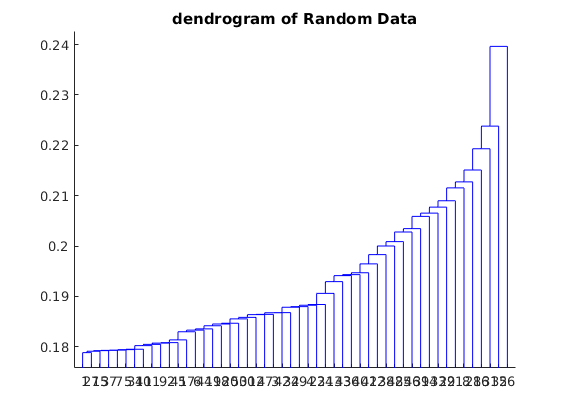
\includegraphics[scale=0.6]{images/clustering/h_random}
%%%%%%%%%%%%%%%%%%%%%%%%%%%%%%%%%%%%%%%%%%%%%%%%%%%%%%%%%%
%%%%%%%%%%%%%%%%%%%%%%%%%%%%%%%%%%%%%%%%%%%%%%%%%%%%%%%%%%
\horizontalLine
\section{Author Contributions}
\label{sec:authorContributions}
\begin{itemize}
    \item Methods:
    \begin{itemize}
        \item Linear Regression: Peggy Li, Steven Mackey, James Dryden
        \item Artificial Neural Networks: Nicholas Layton, Michael Fiueroa
        \item K-Means Clustering: William Otwell, Marshall Hampson, Amos Too
    \end{itemize}
\end{itemize}
\end{document}

